	\section{Leaving Europe}
	In this section we are going to look at the general development throughout the whole world, based on some real-life reports and methods to compare gender affinity between countries, of course with special focus on womens graduation in STEM.
	
	\subsection{Measuring global development - \\The Gender Gap Index}
	
	\subsubsection{Definition}
	
	Where no single measure can capture the complete situation, the Global Gender Gap Index seeks to measure one important aspect of gender equality: \textbf{The relative gaps between women and men across four key areas.}
	The four key areas are: \cite{tgender}
	\begin{itemize}
		\item health and survival
		\item education
		\item economic participation
		\item political empowerment
	\end{itemize}
	The global Gender Gap Index was introduced in 2006 to track progress over time in terms of these 4 categories and the respective differences between women and men. The core idea behind this evaluation is to identify gaps and giving the opportunity to perceive and set the necessary measures to counter or to be more precise close them. In other words, the rankings are designed to raise global awareness of the challenges posed by gender gaps and the opportunities created by reducing them. In 2017, 144 countries have been analyzed annually and the number is constantly growing.
	
	\subsubsection{Gender Gap in Stem Graduates}
	\begin{figure}[h]
		\centering
		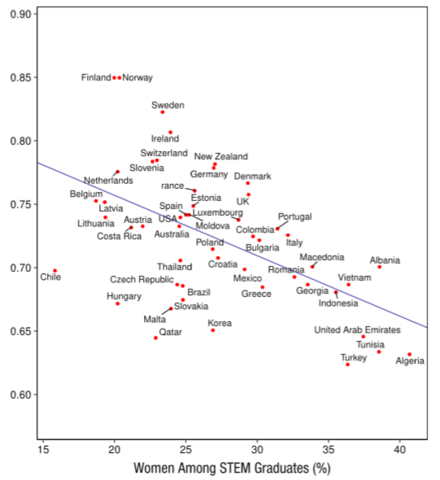
\includegraphics[width=0.9\linewidth]{gender-index-shit}
		\caption[Women among stem graduates]{Women amog STEM graduates worldwide \cite{tgender}}
		\label{fig:gender-index-shit}
	\end{figure}
	Figure \ref{fig:gender-index-shit} points out two important values, that on first sight may not have that much in common. On the x-axis the graduating women amongst all students in STEM topics in percent are displayed, while on the y-axis the Gender-Gap-Index value (as explained in the following chapter) is displayed. The percentage of women with degrees in STEM fields was lower in more gender equal countries (higher Index value on y-axis), as you can see for example in Finland or Norway, where the value was approximately 20\%. In the reverse conclusion, the percentage of women with degrees in countries with lower gender equality the percentage is doubled, as for example in Algeria, Tunisia or Turkey. \cite{tgenderpaper2}\\
	The university of Helsinki in Finland has made a study on this topic, trying to make sense of this trend. They have found out that this phenomenon may have its source in a cultural foundation. In societies where equality in the most fields is given, women tend to stick to more traditional roles, as they don't have to establish that much reputation or proof that they are valuable. On the other hand in less advanced (in terms of gender equality) countries, women try to gain reputation and this leads often to the STEM-topics.
	
	\subsubsection{Quality and Representativity}
	When it comes to reliability on the results of the Gender Gap Report the opinions are divided. In general the team behind the Gender Gap Report uses hundreds of very specific questions and features that they try to evaluate for every country in their program. A thoroughly plausible possibility to screen a wide field of variables.\\
	\newline
	But looking beyond the numbers is extremely important and may change the whole value of the report. The gender gap report is widely used by universities, media organizations, businesses and governments \cite{tgender}. The question is how can one blindly follow or trust an index without deeply analyzing the background of how it has been created. \cite{tagainstgender}.\\
	
	For example, the report does not take into account if women are actually better placed in some key-points than man. The general scale is from 0 to 1, where 0 means inequality and 1 means equality. If women have better results in one key aspect the best measurement that can be reached is 1, but not a value greater than one. As a result: if women are better in 9 out 10 key points the end result is, that they are valued as disadvantaged, because the mean value can therefore only be smaller than 1 and never exactly 1. It is therefore not even possible to reach total equality and a big point of criticism. \cite{tgenderPaper}\\
	\newline
	Another point is, that as stated in \cite{tgenderPaper} certain values are just rare estimations of the real exact state, because of difficult political situations in certain countries all over the world.
	
	\subsection{Investigating the gaps cause}
	So what explains the tendency for nations that have traditionally less gender equality to have more women in science and technology than their gender-progressive counterparts do?\\
		
	It could have to do with the fact that women in countries with higher gender inequality are simply seeking the clearest possible path to financial freedom. And often, that path leads through stem professions.
	
	The issue does not appear to be a girls aptitude for stem professions in general. In looking at test scores across 67 countries and regions researchers found out that girls performed about as well or better than boys did on science in most countries, and in almost all countries, girls would have been capable of college-level science and math classes if they had enrolled in them.\\
	
	Looking at test scores from about 70 countries and regions researchers found out that girls performed about as well or better than boys in most countries.
		
	But when it comes to their relative strengths, in almost all the countries— boys’ best subject was science, and girls’ was reading. (That is, even if an average girl was as good as an average boy at science, she was still likely to be even better at reading.)\\
	\newline
	Across all countries, 24 percent of girls had science as their best subject, 25 percent of girls’ strength was math, and 51 percent excelled in reading. For boys, the percentages were 38 for science, 42 for math, and 20 for reading. And the more gender-equal the country, as measured by the World Economic Forum’s Global Gender Gap Index, the larger this gap between boys and girls in having science as their best subject.
	
	\subsection{Example USA}
	
	"I remember walking into one of the classes at Stanford and just deciding not to take the class because I was one of only three women there, and I just felt so intimidated"\cite{tusa1}\\
	\textit{Catherina Xu – president Women’s Computer Science Society at Stanford University}
	\newline
	
	This is an experience that is widely seen all across the country and one main reason is the lack of women in the field. This development has lead to a shortage of computer science majors.
	
	The percentage of women in the field has been declining since the 1980s. The National Science Foundation found that in 1985, more than 35\% of computer science majors were women. By 2014, that number had dropped down to just 18\%.\\
	
	Laura Adolfie, the Florida STEM Chair for the American Association of University Women, believes part of the problem often starts in childhood. “When a child is born and you have a son or a daughter, they’re socialized by the parents and the grandparents. You tend to give a little girl a doll and a boy cars and things like that.” \cite{tusa1} She said boys are socialized to tinker, which can start them on a path to engineering and computer science.\\
	\newline
	This is one important point, that shows that the general problem begins actually way before studying at the university and graduation. The three key factors for the lack of women in STEM topics are culture, the way women think and a lack of representation in the industry.
	
	\subsection{Example Africa}
	Moving to another continent shows that the general problems are similar to the rest of the world. The cause though may be a different one.\\
	
	For instance in Kenya, out of the top 100 best performing students only 17 were girls, and they were mostly from high-cost national secondary schools. \cite{tafrica1} The statistic worsens as we go down to low-cost district secondary schools.\\
	
	As we heard before the core of the problem lies also in the pre-university education.
	The university of Nairobi did an evaluation where they found out that especially the didactic skills of the teachers and general quality of the classes drastically affect the interest of students in STEM topics. The worse the teacher is, the lower the interest is in STEM topics, affecting more female students because of their different approach of learning \cite{tafrica1} \cite{tchina1}.
	
	\section{Conclusion}
	Gender equality and the empowerment of women and girls will make a crucial contribution to economic development of the world, and STEM education has a big role to play. The current status (globally seen) is  developing in a good direction, but the work is not done yet. As we have seen, the gap in graduations between women and men and general attendance of women in STEM topics has its foundation both in the cultural and political fields and it is the duty of politicians, the society and of course the universities and companies and their staff to create a better and more open environment for education as well as in work and research fields.